\section{Tool}
\label{cp6:tool}


To assist a participant locate text containing information potentially helpful to their tool-supported task, we have developed a proof-of-concept web-browser plug-in 
that highlights text that a semantic-based technique 
identifies as relevant in the artifacts inspected by a participant.



The tool---\acs{beskar} (BERT task-relevant text identifier)---applies 
one of the most promising semantic-based techniques that we have previously explored and evaluated,
i.e., the BERT technique (Chapter~\ref{ch:identifying}),
to identify 10 sentences that are likely relevant to an input task. 
As Figure~\ref{fig:tool-output} shows,
\acs{beskar} highlights the text it automatically identified as relevant 
to a task in a web page under inspection
so that a developer can more easily locate such text.


As a proof-of-concept, we do not focus on the tool's performance.
Therefore, we pre-cached the output 
for the text identified by \acs{beskar} in each task and artifact 
in our experiment. 




\begin{figure}
    \centering
    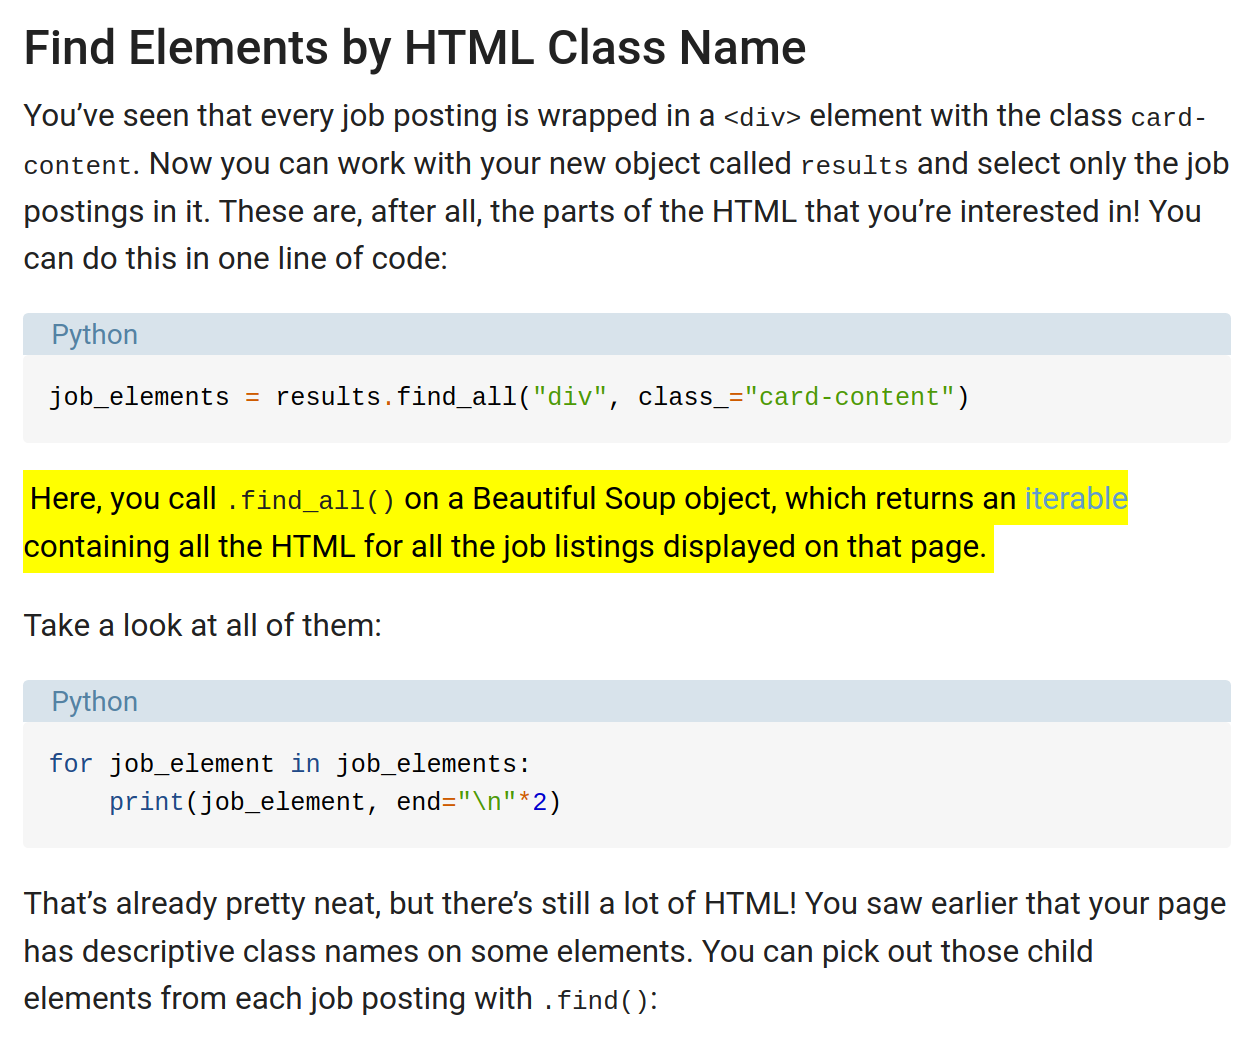
\includegraphics[width=0.85\textwidth]{cp6/tool-highlights.png}
    \caption{Example of a highlight (in yellow) automatically identified by \acs{beskar}
    in a web tutorial pertinent to the NYTimes task}
    \label{fig:tool-output}
\end{figure}

